\documentclass{beamer}
\usetheme{Boadilla}
\usepackage[utf8]{inputenc}
\usepackage{booktabs}
\usepackage{threeparttablex}
\usepackage{mathpazo}
\usepackage[mathpazo]{flexisym}
\usepackage{array}
\usepackage{caption}
\captionsetup[figure]{font=scriptsize}
\usepackage{graphicx}
\usepackage{threeparttablex}
\usepackage[labelformat=empty]{subfig}
\usepackage[T1]{fontenc}
\usepackage{tikz}

\newcommand\hd[2]{\multicolumn{2}{c}{\begin{tabular}{@{}c@{}}#2\end{tabular}}}
\newcolumntype{C}[1]{>{\centering\let\newline\\\arraybackslash\hspace{0pt}}m{#1}}
\let\estinput=\input
\newcommand{\estwide}[3]{
        \vspace{.75ex}{
            \textsymbols
            \begin{tabular*}
            {\textwidth}{@{\hskip\tabcolsep\extracolsep\fill}l*{#2}{#3}}
            \toprule
            \estinput{#1}
            \bottomrule
            \addlinespace[.75ex]
            \end{tabular*}
            }
        }

\newcommand{\estauto}[3]{
        \vspace{.75ex}{
            \textsymbols
            \begin{tabular}{l*{#2}{#3}}
            \toprule
            \estinput{#1}
            \bottomrule
            \addlinespace[.75ex]
            \end{tabular}
            }
        }

\newcommand{\specialcell}[2][c]{%
    \begin{tabular}[#1]{@{}c@{}}#2\end{tabular}
}

\definecolor{MyBackground}{rgb}{0.95,0.95,0.96}
\setbeamercolor{background canvas}{bg=MyBackground}

\definecolor{UniBlue}{RGB}{83,121,170}
\setbeamercolor{title}{fg=UniBlue}
\setbeamercolor{frametitle}{fg=UniBlue}
\setbeamercolor{structure}{fg=UniBlue}
\setbeamertemplate{footline}{}

\AtBeginSection[]{
  \begin{frame}
  \vfill
  \centering
  \begin{beamercolorbox}[sep=8pt,center,shadow=true,rounded=true]{title}
    \usebeamerfont{title}\insertsectionhead\par%
  \end{beamercolorbox}
  \vfill
  \end{frame}
}

\title[]{Project Workflow}
\date{}

\begin{document}

\maketitle

\beamertemplatenavigationsymbolsempty
\begin{frame}{Project Workflow - Motivation}
    \begin{figure}
        
\includegraphics[scale=0.35]{clutter.jpeg}
    \end{figure}      
\end{frame}

\begin{frame}{Project Workflow - Automation}
    \begin{itemize}
        \item Gentzkow and Shapiro (2014): Automation
            \begin{itemize}
                \item Automate everything that can be automated.
                \item Write a single script that executes all code from beginning to end.
            \end{itemize}
        \bigskip
        \item Application:
            \begin{itemize}
                \item README file
                \item Master script file
            \end{itemize}
    \end{itemize}
\end{frame}

\begin{frame}{Automation - README File}
    \begin{itemize}
        \item Purpose: orientation and instruction
            \begin{itemize}
                \item Start Here
            \end{itemize}
        \medskip
        \item Contents:
            \begin{itemize}
                \item Project description
                \item Instructions for replication (master script file)
                \item Instructions for data access
                \item Special considerations for software prep (e.g., user written Stata commands)
            \end{itemize}
        \medskip
        \pause\item Example:
            \begin{itemize}
                \item \color{blue} \href{https://github.com/hollina/macroeconomic_conditions_and_opioid_abuse}{Hollingsworth, A., Ruhm, C. J., \& Simon, K. (2017). Macroeconomic Conditions and Opioid Abuse. Journal of Health Economics, 56, 222–233.}
            \end{itemize}
    \end{itemize}
\end{frame}

\begin{frame}{Automation - Master File}
    \begin{itemize}
        \item Purpose: single project file that runs all individual project files
            \begin{itemize}
                \item Roadmap for the analytic process
            \end{itemize}
        \medskip
        \item Contents:
            \begin{itemize}
                \item Series of well-annotated statements that run script files for data cleaning, analysis, table/figure creation, etc.
                \item Includes commands to clear output files/tables/figures.
            \end{itemize}
        \medskip
        \pause\item Example:
            \begin{itemize}
                \item \color{blue} \href{https://github.com/k-callison/hpam7660-sp24/blob/main/resources/agb_masterfile.pdf}{Goodman-Bacon, A. (2021). The Long-Run Effects of Childhood Insurance Coverage: Medicaid Implementation, Adult Health, and Labor Market Outcomes. American Economic Review, 111(8): 2550-93.}
            \end{itemize}
    \end{itemize}
\end{frame}

\begin{frame}{Project Workflow - Version Control}
    \begin{itemize}
        \item Gentzkow and Shapiro (2014): Version Control
            \begin{itemize}
                \item Store code and data under version control.
                \item Run the whole directory before checking it back in.
            \end{itemize}
        \medskip
        \item Application:
            \begin{itemize}
                \item File repository (GitHub)
            \end{itemize}
    \end{itemize}
\end{frame}

\begin{frame}{Project Workflow - Version Control}
    \begin{itemize}
        \item Purpose: avoid this
            \begin{figure}
                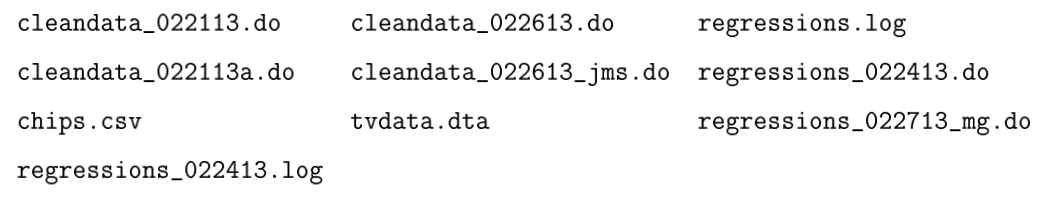
\includegraphics[scale=0.55]{files.png}
            \end{figure}
        \bigskip
        \item How it works:
            \begin{itemize}
                \item Maintain one file (e.g., regressions.log).
                \item File changes are tracked each time the file is "checked back in" (i.e., commit changes and push to GitHub).
                \item If you screwed up, revert back to the previous commit.
            \end{itemize}
    \end{itemize}
\end{frame}

\begin{frame}{Project Workflow - Version Control}
    \begin{figure}
        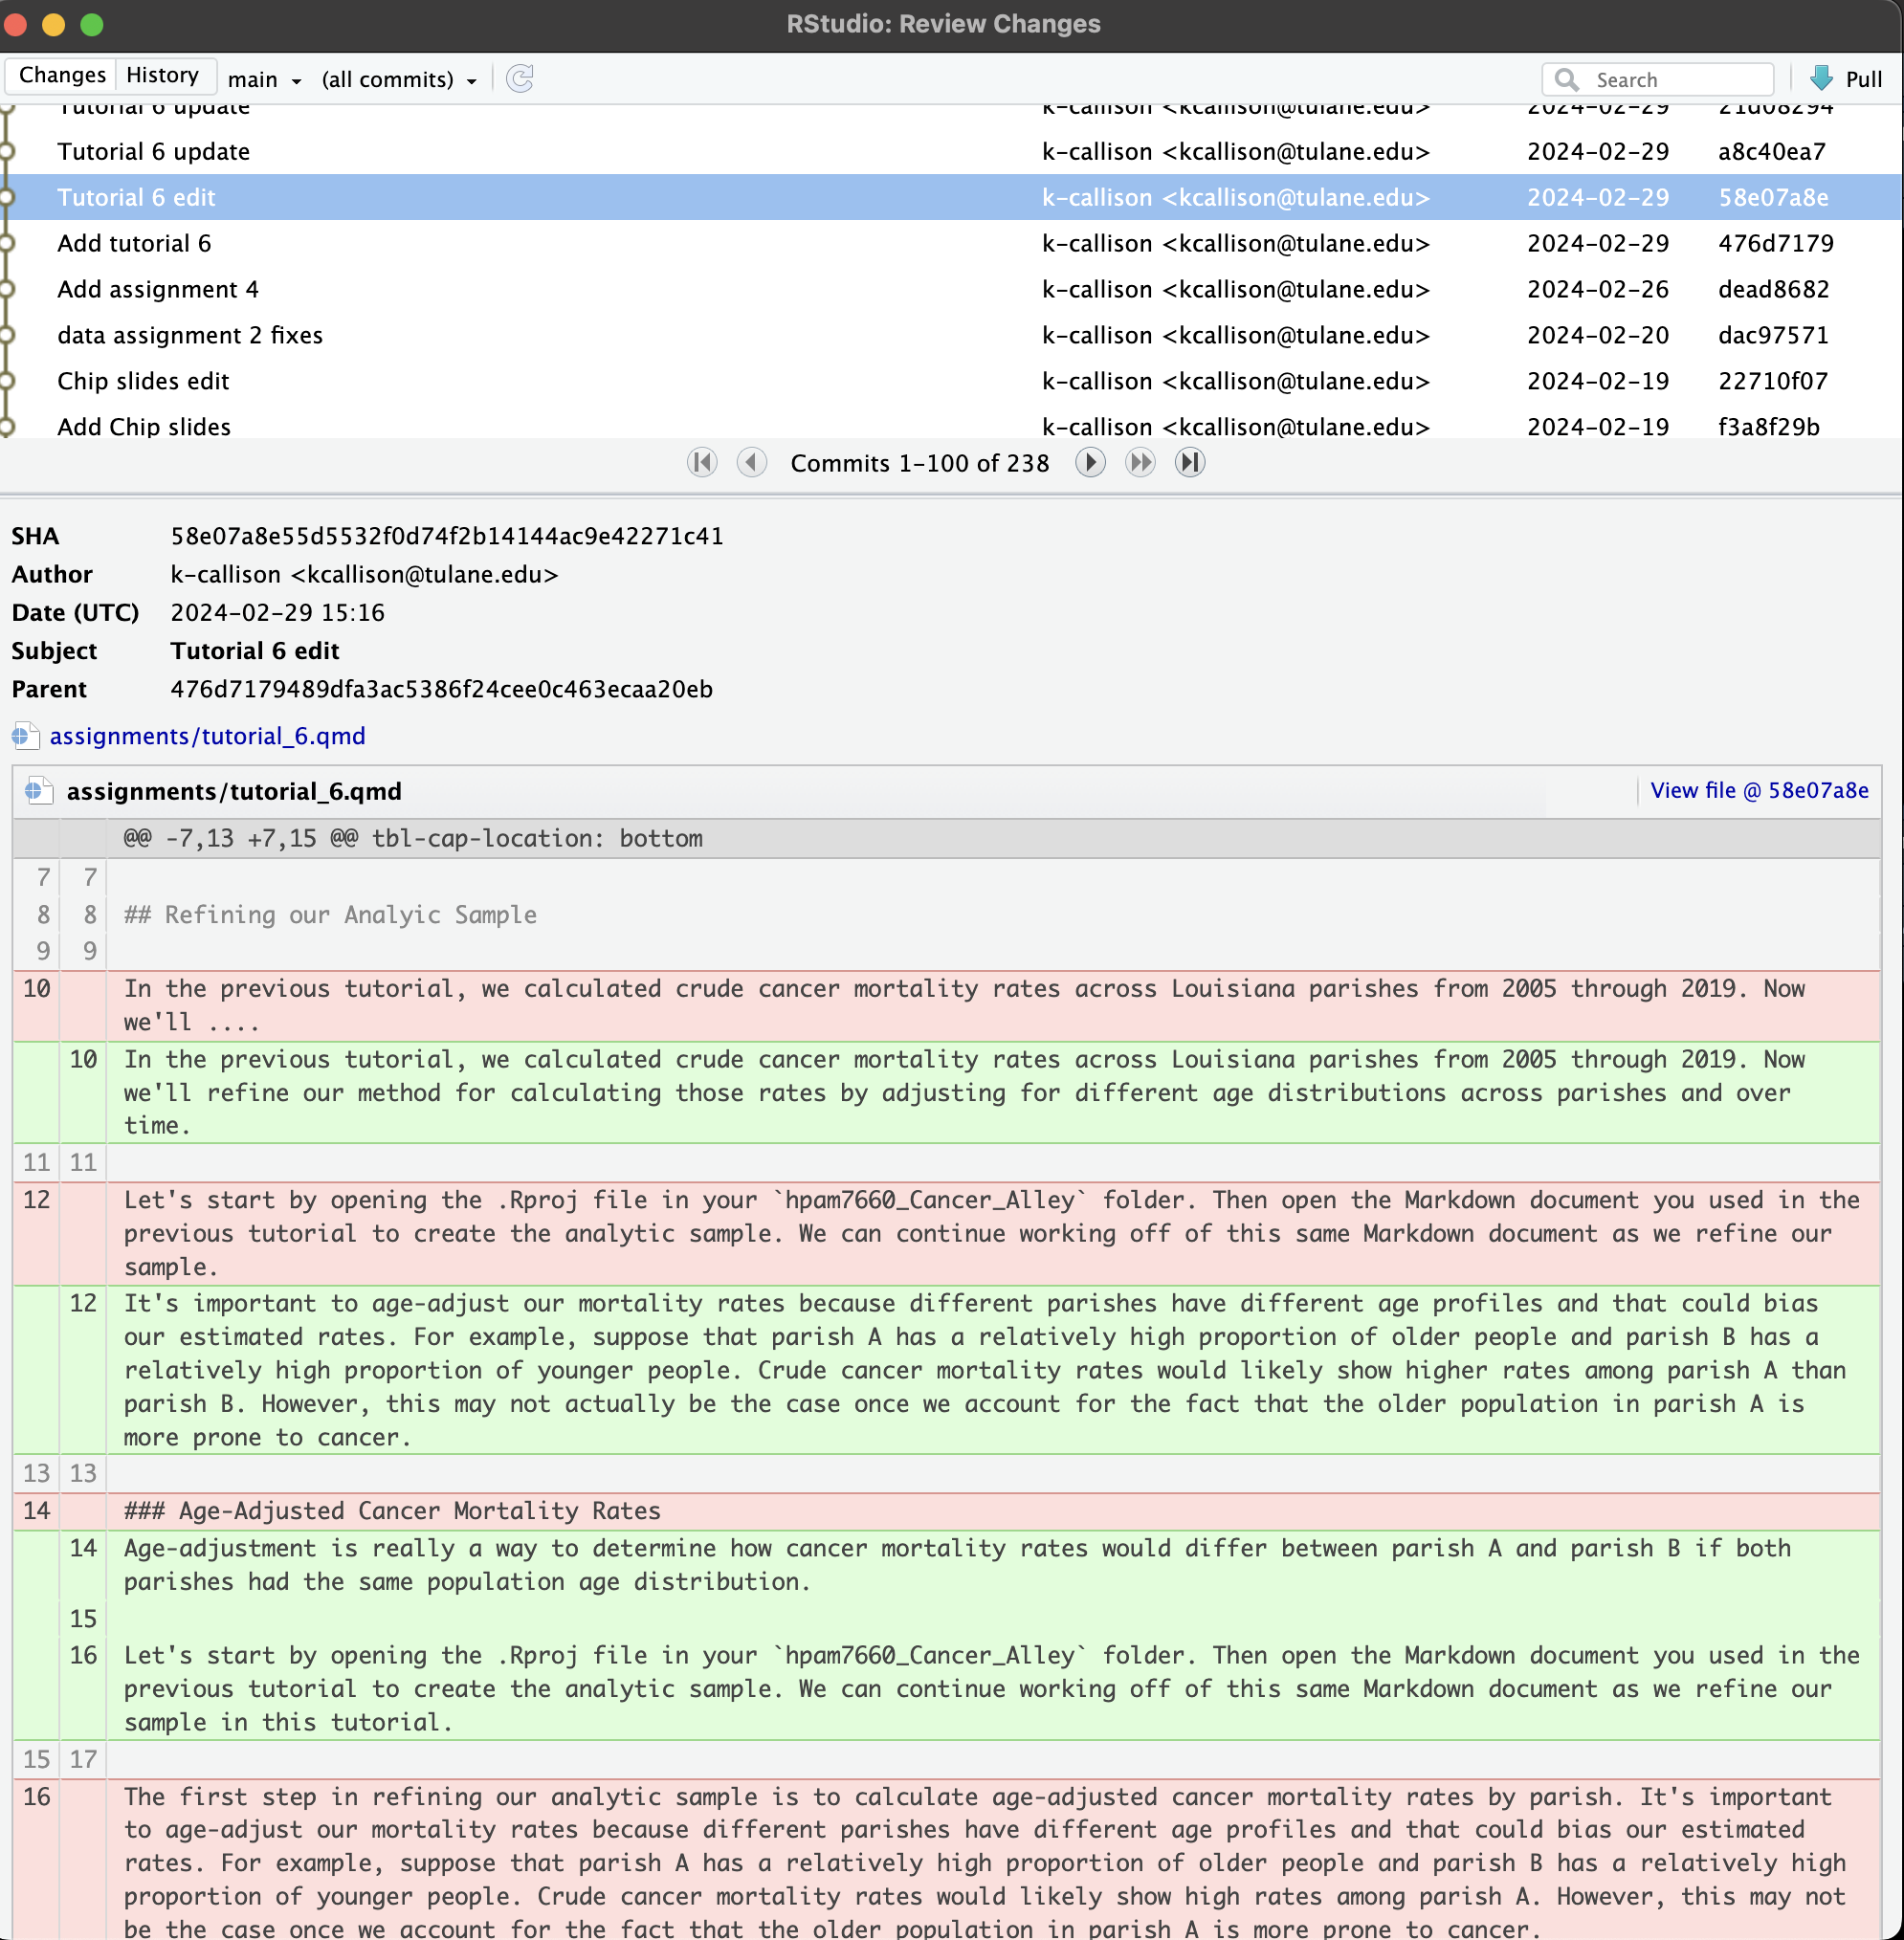
\includegraphics[scale=0.25]{version_control.png}
    \end{figure}    
\end{frame}

\begin{frame}{Project Workflow - Version Control}
    \begin{itemize}
        \item Gentzkow and Shapiro (2014): Version Control
            \begin{itemize}
                \item Store code and data under version control.
                \item \textbf{Run the whole directory before checking it back in.}
                    \begin{itemize}
                        \item[-] \textbf{Run your master file before each push.} 
                    \end{itemize}
            \end{itemize}
        \medskip
        \item Application:
            \begin{itemize}
                \item File repository (GitHub)
            \end{itemize}
    \end{itemize}
\end{frame}

\begin{frame}{Project Workflow - Directory Management}
    \begin{itemize}
        \item Gentzkow and Shapiro (2014): Directories
            \begin{itemize}
                \item Separate directories by function.
                \item Separate files into inputs and outputs.
                \item Make directories portable.
            \end{itemize}
        \medskip
        \item Application:
            \begin{itemize}
                \item Directory map in your README file
            \end{itemize}
    \end{itemize}
\end{frame}

\begin{frame}{Project Workflow - Directory Management}
    \begin{itemize}
        \item Gentzkow and Shapiro directory map:
    \end{itemize}
    \begin{figure}
        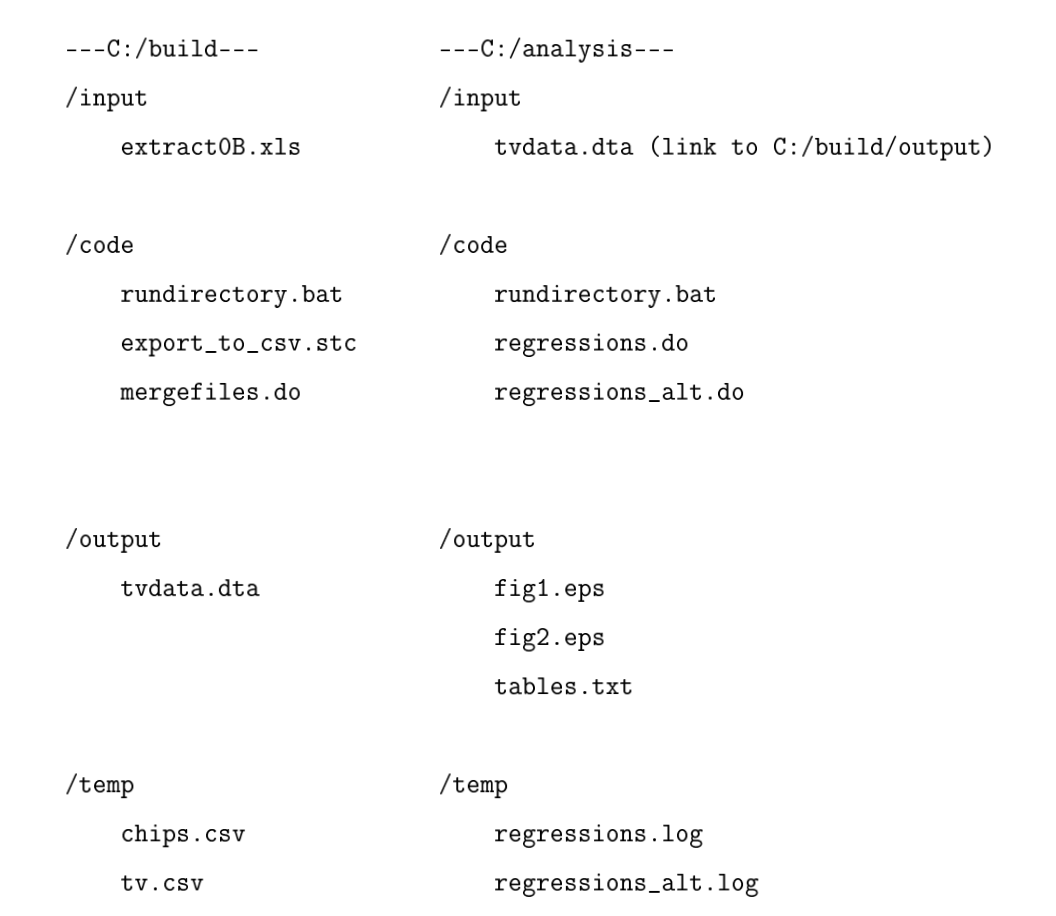
\includegraphics[scale=0.43]{GS_directory.png}
    \end{figure}    
\end{frame}

\begin{frame}{Project Workflow - Directory Management}
    \begin{itemize}
        \item Goodman-Bacon directory map:
    \end{itemize}
    \begin{figure}
        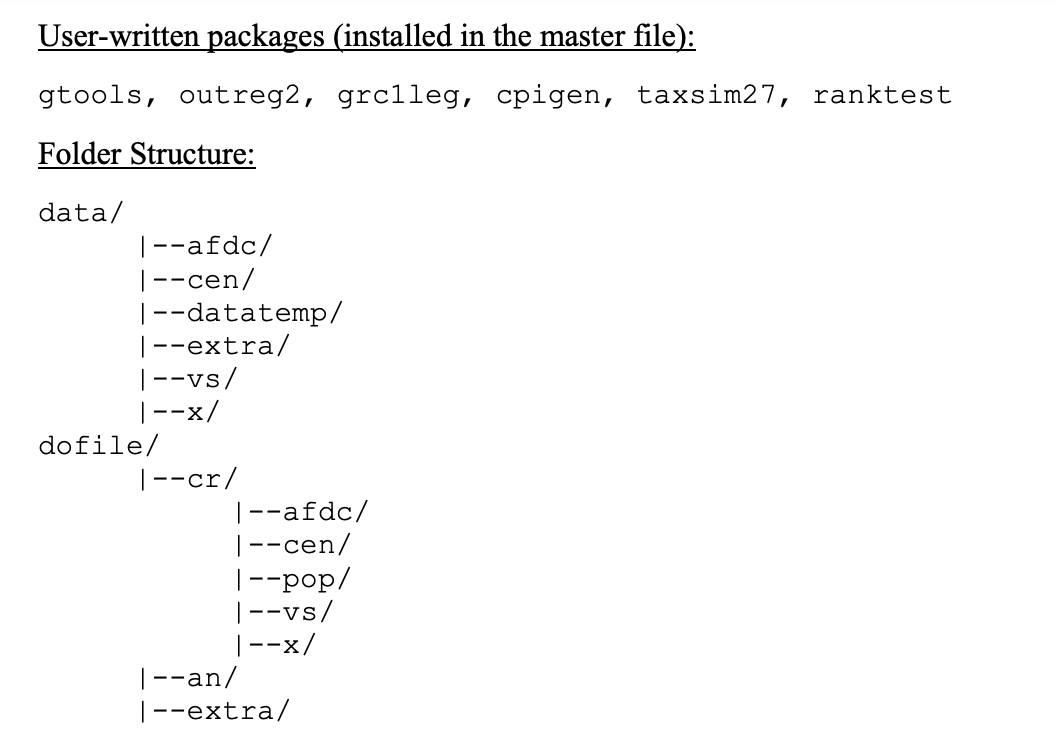
\includegraphics[scale=0.43]{agb_directory.png}
    \end{figure}    
\end{frame}

\begin{frame}{Project Workflow - Directory Management}
    \begin{itemize}
        \item Example directory map:
    \end{itemize}
    \begin{figure}
        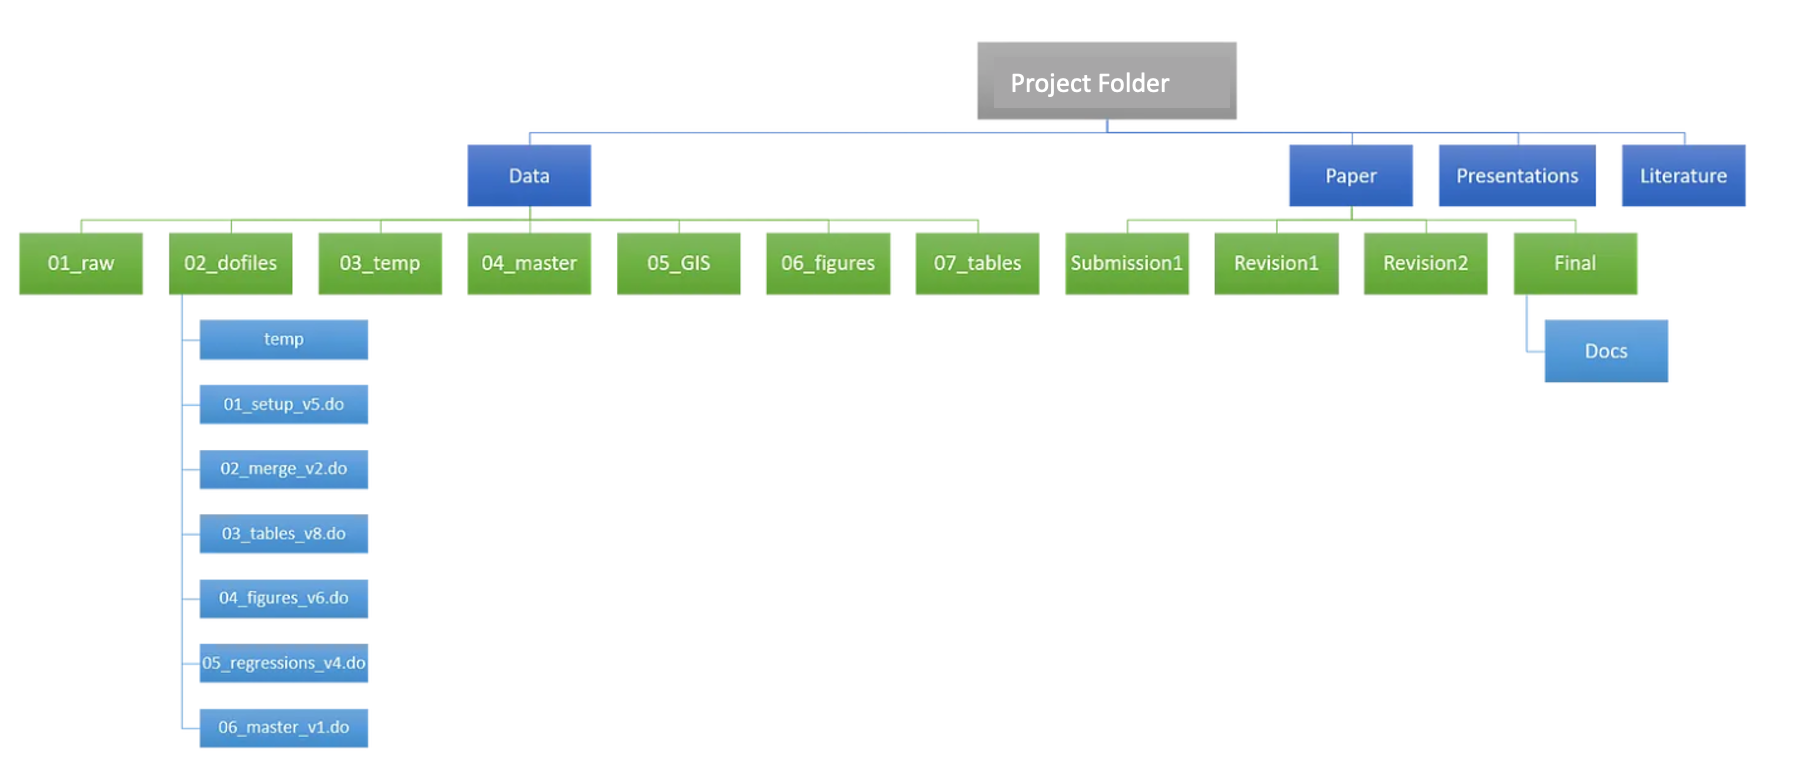
\includegraphics[scale=0.37]{directory_flow.png}
    \end{figure}    
\end{frame}

\begin{frame}{Project Workflow - Directory Management}
    \begin{itemize}
        \item Navigating directories (Stata example):
    \end{itemize}
    \begin{figure}
        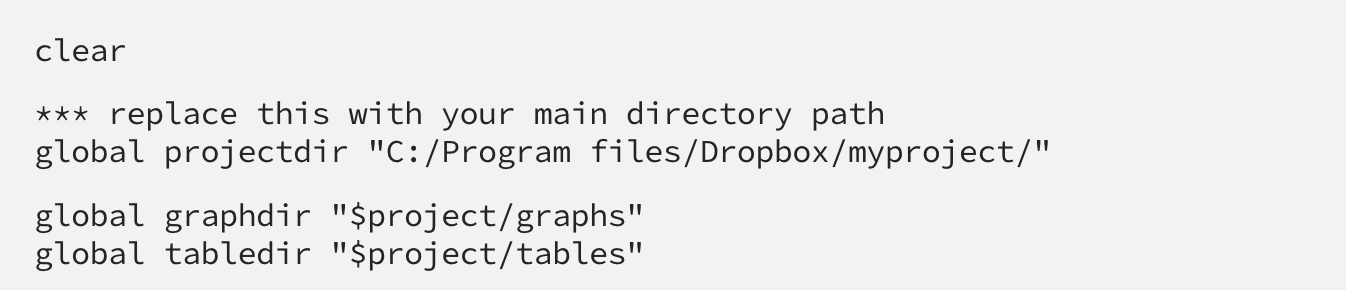
\includegraphics[scale=0.5]{globals.png}
    \end{figure}  
        \bigskip
    \begin{itemize}
        \pause\item Note: be carefule using globals to define lists of control variables when using multiple .do files.
    \end{itemize}  
\end{frame}

\begin{frame}{Project Workflow - Project Management}
    \begin{itemize}
        \item Gentzkow and Shapiro (2014): Management
            \begin{itemize}
                \item Manage tasks with a task management system.
                \item Email is not a task management system.
        \end{itemize}
        \medskip
        \item Application:
            \begin{itemize}
                \item GitHub Issues and Task Lists
            \end{itemize}
    \end{itemize}
\end{frame}

\begin{frame}{Project Workflow - Project Management}
    \begin{figure}
        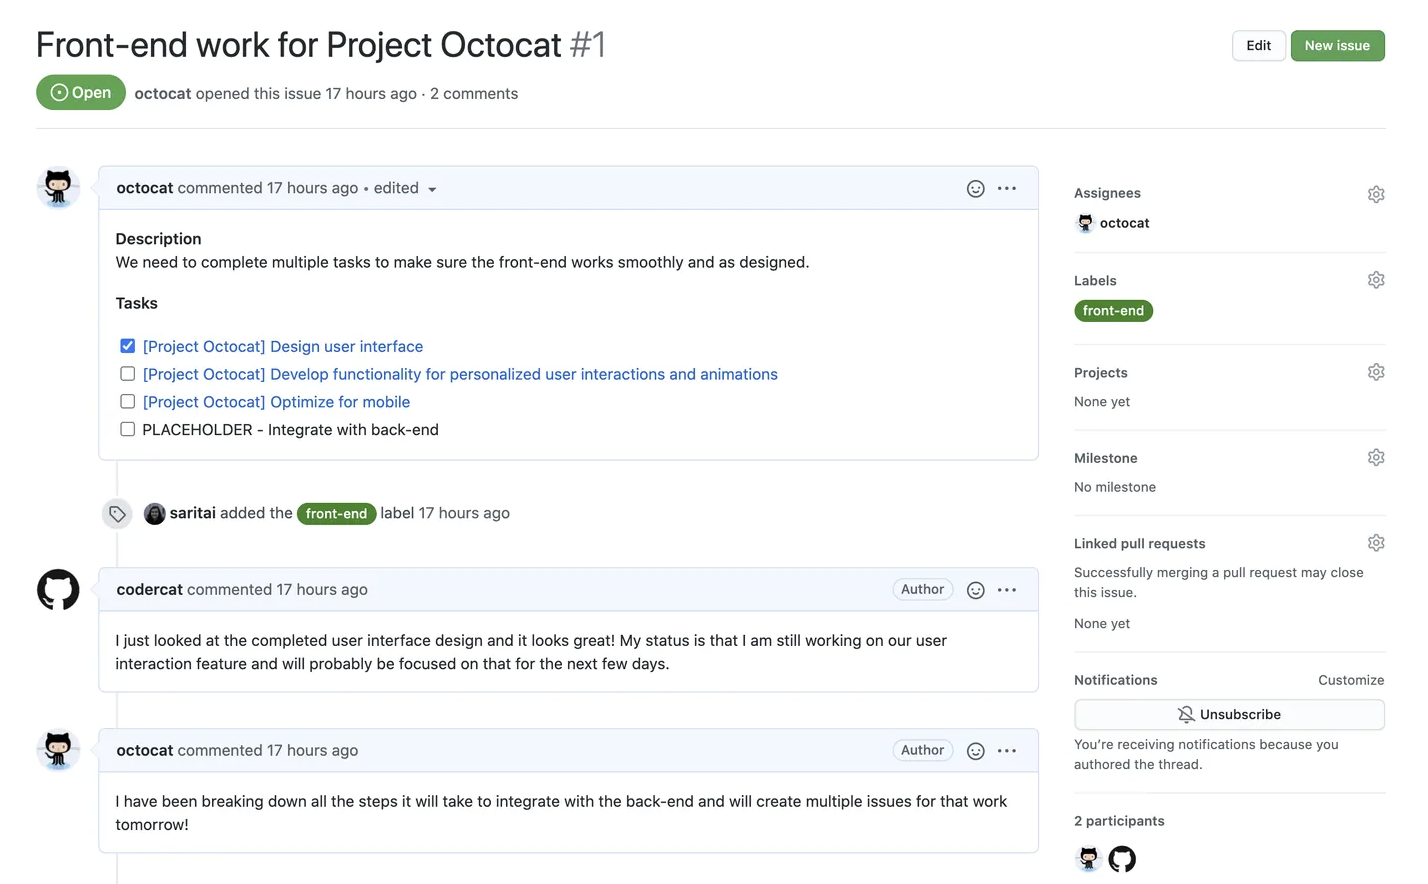
\includegraphics[scale=0.45]{manage.png}
    \end{figure}    
\end{frame}

\begin{frame}{Project Workflow - Tools}
    \begin{itemize}
        \item Tools for an efficient project workflow:
        \smallskip
            \begin{itemize}
                \item Statistical software: R or Stata
                \smallskip
                \item Word processing software: LaTeX (Markdown/Quarto)
                \smallskip
                \item Integrated development environment (IDE): RStudio or Visual Studio Code (VS Code)
                \smallskip
                \begin{itemize}
                    \item[-] Stata isn't great for this
                \end{itemize}
                \smallskip
                \item Version control: Git and GitHub
            \end{itemize}
        \end{itemize}
\end{frame}

\end{document}
